\documentclass[a4paper,12pt]{article}
\usepackage[english,ukrainian,russian]{babel}
\linespread{1}
\usepackage{ucs}
\usepackage[utf8]{inputenc}
\usepackage[T2A]{fontenc}
\usepackage[paper=portrait,pagesize]{typearea}
\usepackage{amsmath}
\usepackage{bigints}
\usepackage{amsfonts}
\usepackage{graphicx}
\usepackage{amssymb}
\usepackage{cancel}
\usepackage{gensymb}
\usepackage{multirow}
\usepackage{rotate} 
\usepackage{pdflscape}
\usepackage{bigstrut}
\usepackage[pageanchor]{hyperref}
\usepackage{chngpage}
\usepackage{fancybox,fancyhdr}
\newcommand\tab[1][1cm]{\hspace*{#1}}
\newcommand{\RomanNumeralCaps}[1]{\MakeUppercase{\romannumeral #1}}
\usepackage[left=20mm, top=20mm, right=15mm, bottom=15mm, nofoot]{geometry}

\usepackage{listings}
\usepackage{xcolor}

\definecolor{codegreen}{rgb}{0,0.6,0}
\definecolor{codegray}{rgb}{0.5,0.5,0.5}
\definecolor{codepurple}{rgb}{0.58,0,0.82}
\definecolor{backcolour}{rgb}{0.95,0.95,0.92}

\lstdefinestyle{mystyle}{
	backgroundcolor=\color{backcolour},   
	commentstyle=\color{codegreen},
	keywordstyle=\color{blue},
	numberstyle=\tiny\color{codegray},
	stringstyle=\color{red},
	basicstyle=\ttfamily\footnotesize,
	breakatwhitespace=false,         
	breaklines=true,                 
	captionpos=b,                    
	keepspaces=true,                 
	numbers=none,                    
	numbersep=5pt,                  
	showspaces=false,                
	showstringspaces=false,
	showtabs=false,                  
	tabsize=4,
	frame=shadowbox
}

\lstset{style=mystyle}

\begin{document}
    \pagestyle{fancy}
    \fancyhead{}
    \fancyhead[R]{ФІ-12 Завалій Олександр}
    \begin{center}
        \large{\textbf{Міністерство освіти і науки України\\
                Національний технічний університет України\\
                «Київський політехнічний інститут імені Ігоря Сікорського»\\
                Навчально-науковий Фізико-технічний інститут}}\\
        \hfill \break \hfill \break \hfill\break \hfill \break \hfill \break \hfill \break \hfill \break
        \hfill \break \hfill \break \hfill \break
        \begin{center}
            \normalsize{\textbf{ОПЕРАЦІЙНІ СИСТЕМИ\\
            Комп’ютерний практикум\\
            Робота №8}}
        \end{center}
    \end{center}
    \hfill \break \hfill \break \hfill \break \hfill \break \hfill \break \hfill \break \hfill \break
    \hfill \break \hfill \break \hfill \break \hfill \break 
    \begin{flushright}
        \large{ \hspace{35pt} Виконав:\\
            студент групи ФI-12\\
            Завалій Олександр\\} 
        \large{ \hspace{35pt} Перевірив:\\
        Кірієнко О.В.} 
    \end{flushright}
    \hfill \break \hfill \break \hfill \break \hfill \break \hfill \break \hfill \break \hfill \break
    \hfill \break
    \begin{center} \textbf{Київ-2023} \end{center}
    \thispagestyle{empty}

\newpage
    \begin{center}
        \section*{\bfseries{Робота №8.\\
        Засоби синхронізації потоків }}
    \end{center}
    \textbf{Мета:} \\
    \hangindent=1.5cm 
    \hangafter=+1 \noindent
    Оволодіння практичними навичками розроблення багатопотокових програм з підтримкою засобів синхронізаці. \\
    \begin{center}
        \Large{Варіант №5}
    \end{center}
    Зміст індивідуального завдання:
    \begin{enumerate}
        \item Розминка. Стандартна задача виробник-споживач. \\
        Задача була розглянута на лекції. Також детально розглянута в рекомендованих книжках [1, 5]. Розробіть
        програму, що демонструє рішення цієї задачі за допомогою семафорів. Для цього напишіть:
        \begin{itemize}
            \item функції виробника і споживача (наприклад, як на лекції, або як у Шеховцові, але так, щоби працювало);
            \item функції створення і споживання об’єктів (рекомендується “створювати” рядки тексту шляхом зчитування їх з файлу,
            хоча можливі й інші варіанти за вибором викладача або за вашою фантазією, наприклад розрахунки геш-функцій
            sha2 з рядків рандомних символів, а “споживати” їх шляхом роздрукування на екрані з додатковою
            інформацією такою як ідентифікатор потоку і мітка часу, причому і там, і там для моделювання складного
            характеру реального життя виробників і споживачів можна додавати рандомні затримки);
            \item функцію main(), що створює потоки-виробники і потоки-споживачі, при цьому треба передбачити введення з
            клавіатури або як параметри командного рядка кількості записів у буфері, кількості виробників і кількості споживачів для досліджень їх роботи;
            \item обов’язково передбачити коректне завершення усього цього господарства.
        \end{itemize}
        Продемонструвати викладачеві як воно працює (не менше двох виробників і двох споживачів) і код, що ви написали.
        \item Продовження розминки. Теж саме, але не на семафорах, а на м’ютексі і умовних змінних. \\
        Модифікуйте програму п. 1 так, щоби використовувати м’ютекс і умовну змінну.
        \item Продовження розминки для тих, хто шукає пригод. Взаємне блокування. \\
        Модифікуйте програму п. 1 так, щоби викликати взаємне блокування. Для цього поміняйте місцями семафори.
        Переконайтесь у факті взаємного блокування і отримайте задоволення.
        \item Індивідуальне завдання. \\
        Варіант 2 в. Філософи, що обідають 3 \\
        Все тотожнє варіанту 2 б, за винятком типу очікування.
        Якщо філософ не може взяти виделку (першу або другу), він має покласти на стіл першу виделку, якщо він її вже
        захопив, і заснути. Реалізувати можна за допомогою додаткових м’ютексів і умовних змінних. Відповідно, коли
        філософ звільнює виделки, він має сигналізувати про це. Чи часто філософи падають в обморок? А якщо час його сну додавати до часу “голодування”?
    \end{enumerate}

\newpage
    \begin{center}
        \Large{Task \RomanNumeralCaps{1}}
    \end{center}
    \textbf{Розминка. Стандартна задача виробник-споживач. \\
    Задача була розглянута на лекції. Також детально розглянута в рекомендованих книжках [1, 5]. Розробіть
    програму, що демонструє рішення цієї задачі за допомогою семафорів.}
    \begin{figure}[h!]
        \begin{minipage}[h]{1\linewidth}
            \centering
            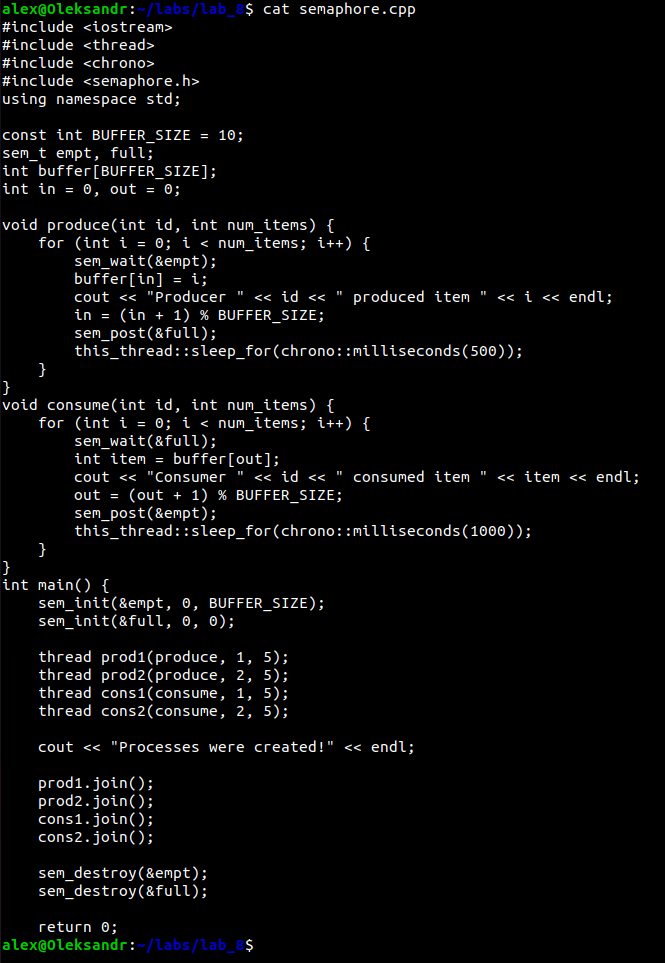
\includegraphics[width=0.8\linewidth]{Prt sc/Figure_1_1.png}  
        \end{minipage}
    \end{figure}

\newpage
    \begin{figure}[h!]
        \begin{minipage}[h]{1\linewidth}
            \centering
            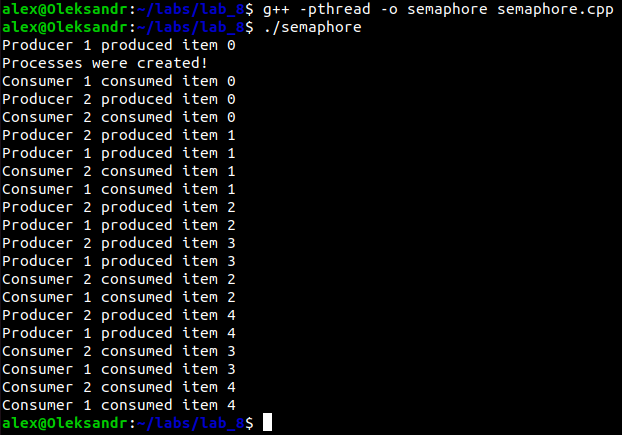
\includegraphics[width=0.8\linewidth]{Prt sc/Figure_1.png}  
        \end{minipage}
    \end{figure}

\newpage
    \begin{center}
        \Large{Task \RomanNumeralCaps{2}}
    \end{center}
    \textbf{Продовження розминки. Теж саме, але не на семафорах, а на м’ютексі і умовних змінних. \\
    Модифікуйте програму п. 1 так, щоби використовувати м’ютекс і умовну змінну.}
    \begin{figure}[h!]
        \begin{minipage}[h]{1\linewidth}
            \centering
            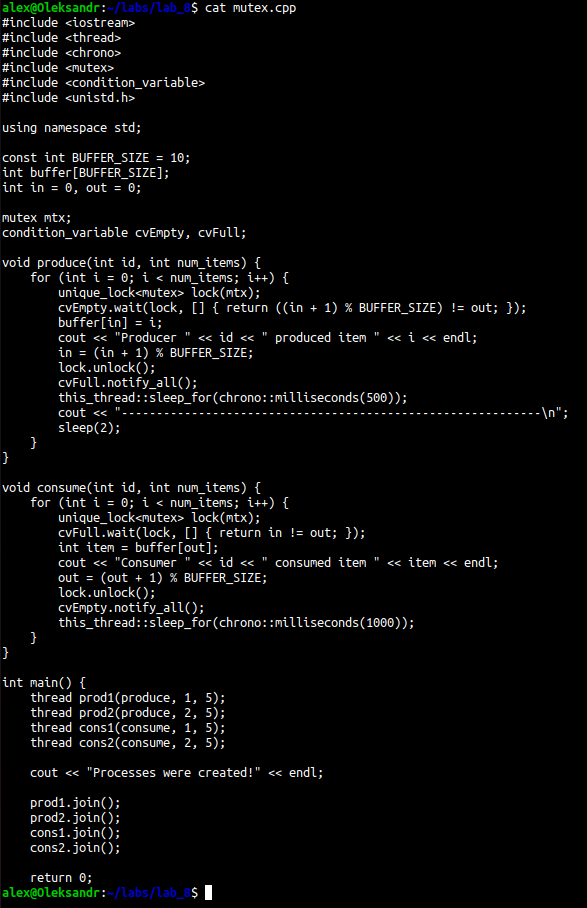
\includegraphics[width=0.8\linewidth]{Prt sc/Figure_2_1.png}  
        \end{minipage}
    \end{figure}

\newpage
    \begin{figure}[h!]
        \begin{minipage}[h]{1\linewidth}
            \centering
            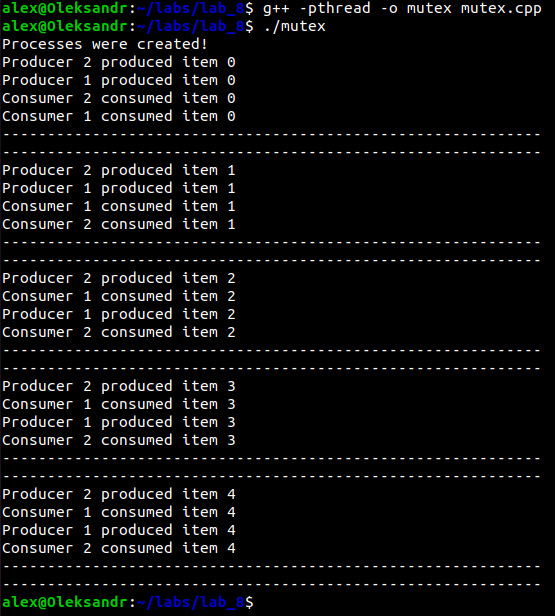
\includegraphics[width=0.8\linewidth]{Prt sc/Figure_2.png}  
        \end{minipage}
    \end{figure}

\newpage
    \begin{center}
        \Large{Task \RomanNumeralCaps{3}}
    \end{center}
    \textbf{Продовження розминки для тих, хто шукає пригод. Взаємне блокування. \\
    Модифікуйте програму п. 1 так, щоби викликати взаємне блокування. Для цього поміняйте місцями семафори.
    Переконайтесь у факті взаємного блокування і отримайте задоволення.}
    \begin{figure}[h!]
        \begin{minipage}[h]{1\linewidth}
            \centering
            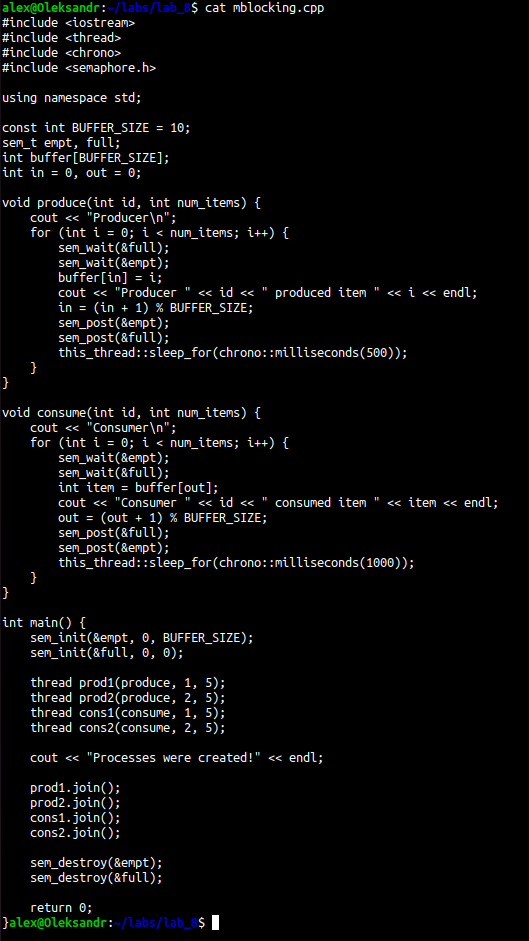
\includegraphics[width=0.7\linewidth]{Prt sc/Figure_3_1.png}  
        \end{minipage}
    \end{figure}

\newpage
    \begin{figure}[h!]
        \begin{minipage}[h]{1\linewidth}
            \centering
            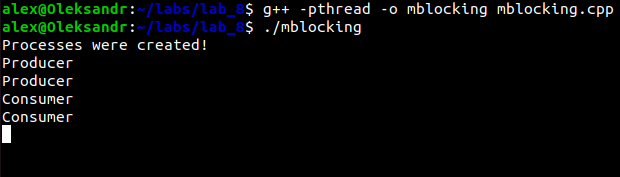
\includegraphics[width=0.8\linewidth]{Prt sc/Figure_3.png}  
        \end{minipage}
    \end{figure}
    \begin{center}
        \Large{Task \RomanNumeralCaps{4}}
    \end{center}
    \textbf{Індивідуальне завдання. \\
    Варіант 2 в. Філософи, що обідають 3 \\
    Все тотожнє варіанту 2 б, за винятком типу очікування.
    Якщо філософ не може взяти виделку (першу або другу), він має покласти на стіл першу виделку, якщо він її вже
    захопив, і заснути. Реалізувати можна за допомогою додаткових м’ютексів і умовних змінних. Відповідно, коли
    філософ звільнює виделки, він має сигналізувати про це. Чи часто філософи падають в обморок? А якщо час його сну додавати до часу “голодування”?}
    \begin{figure}[h!]
        \begin{minipage}[h]{1\linewidth}
            \centering
            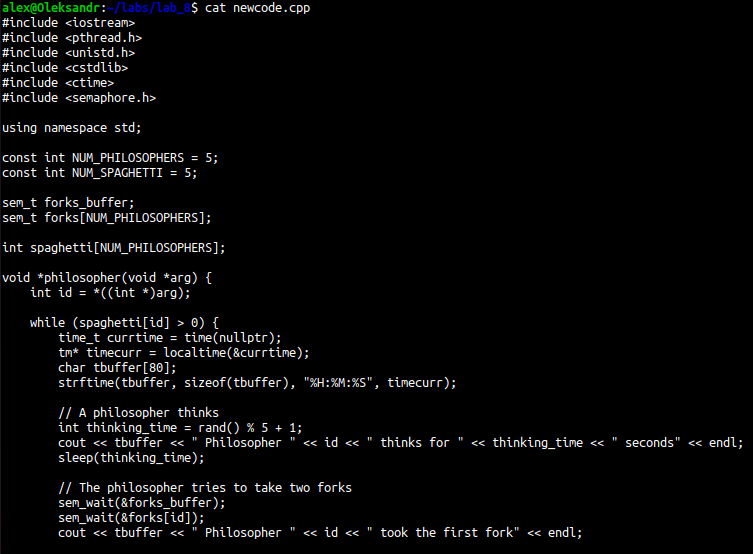
\includegraphics[width=0.8\linewidth]{Prt sc/Figure_4_1.png}  
        \end{minipage}
    \end{figure}

\newpage
    \begin{figure}[h!]
        \begin{minipage}[h]{1\linewidth}
            \centering
            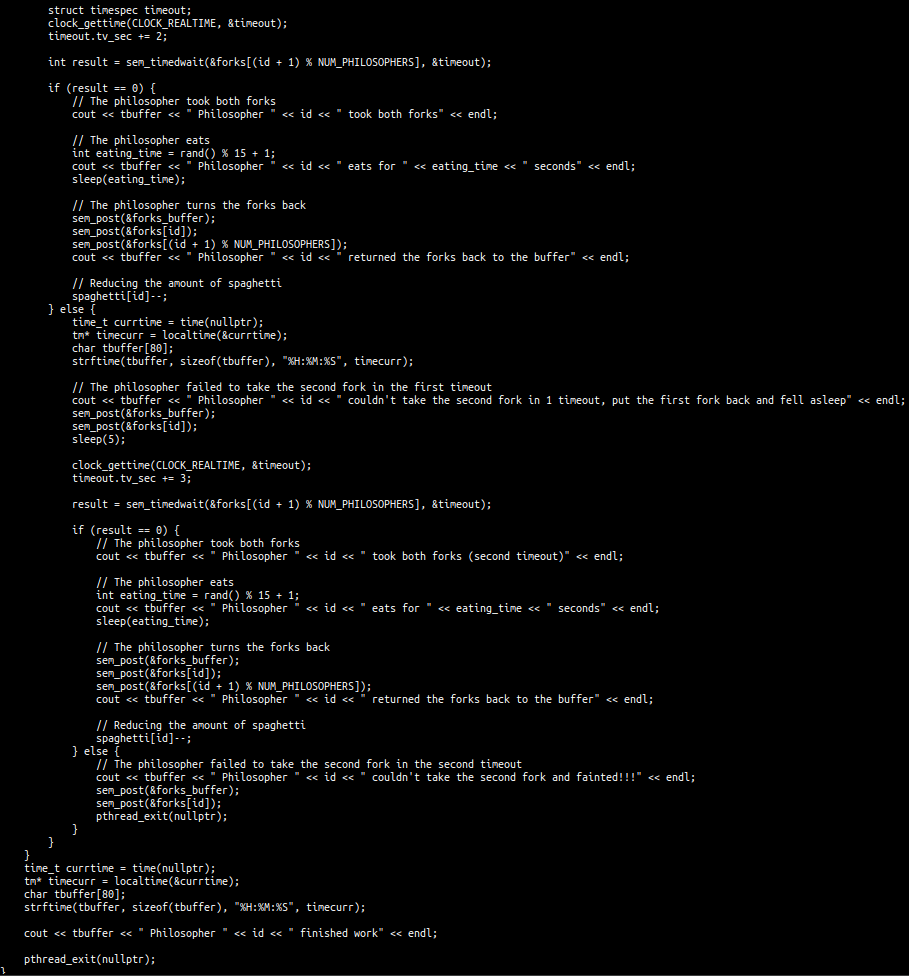
\includegraphics[width=0.8\linewidth]{Prt sc/Figure_4_2.png}  
        \end{minipage}
    \end{figure}
    \begin{figure}[h!]
        \begin{minipage}[h]{1\linewidth}
            \centering
            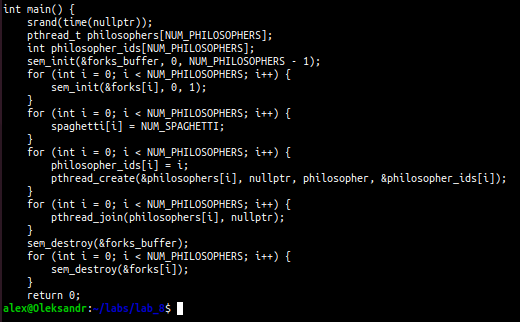
\includegraphics[width=0.8\linewidth]{Prt sc/Figure_4_3.png}  
        \end{minipage}
    \end{figure}

\newpage
    \begin{figure}[h!]
        \begin{minipage}[h]{1\linewidth}
            \centering
            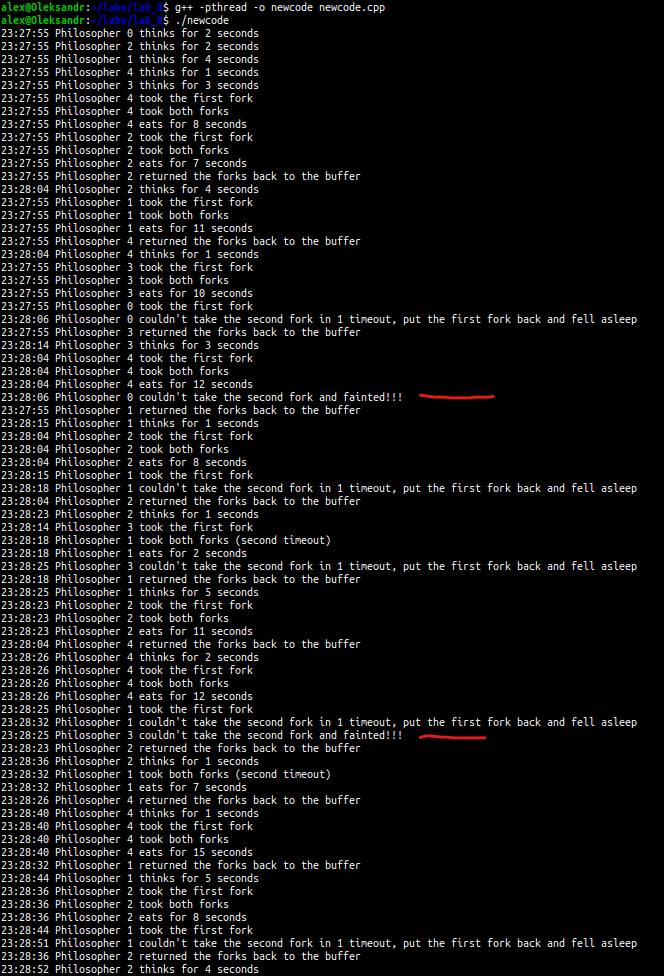
\includegraphics[width=0.8\linewidth]{Prt sc/Figure_4.png}  
        \end{minipage}
    \end{figure}
    На скріншоті видно, що на п'ять філософів двоє впали в обморок. Також перший процес міг завершитись три рази, але йому пощастило більше.
    Тобто філософи часто падають в обморок, оскільки веделок всього п'ять. Отже виходить одночасно їсти може лише двоє, а інші в цей час думають.
    Також це буде залежить від часу за який філософи їдять. Оскільки це число випадкове, то відповідно два філософи можуть їсти довше, аніж інші три думають.
    Якщо час сну додавати до часу "голодування", то вийде що деякі філософи, в теорії, можуть весь час "голодувати". Адже веделки заберає той потік, що перший отримує доступ
    до буферу. Тому якщо потоків багато, а веделок мало, можемо виникнути ситуації коли потоки будуть чекати доки інші завершать своє виконання і тільки після цього отримають доступ.

\newpage
    \begin{center}
        \Large{Висновки}
    \end{center}

    Оволодіння практичними навичками розроблення багатопотокових програм з підтримкою засобів синхронізації набирує актуальності. 
    Оскільки у сучасному світі, де швидкість і ефективність програмного забезпечення мають ключове значення, уміння розробляти багатопотокові 
    програми знаходить широке застосування.

    Потокам та процесам часто потрібно взаємодіяти один з одним, наприклад, один процес може передавати дані іншому процесу, або декілька процесів можуть обробляти 
    дані із загального файлу. У всіх цих випадках виникає проблема синхронізації процесів, яка може вирішуватися припиненням і активізацією процесів, організацією черг, блокуванням і звільненням ресурсів.

    Якщо розбиратись детальніше, то механізмами синхронізації є засоби операційної системи, які допомагають розв'язувати основне завдання синхронізації — забезпечувати 
    координацію потоків, які працюють зі спільно використовуваними даними. Якщо такі засоби — це мінімальні блоки для побудови багатопотокових програм, 
    їх називають синхронізаційними примітивами. 

    Їх поділяють на такі основні категорії:
    \begin{enumerate}
        \item універсальні, низького рівня, які можна використовувати різними способами (семафори);
        \item прості, низького рівня, кожен з яких пристосований до розв'язання тільки однієї задачі (м'ютекси та умовні змінні);
        \item універсальні високого рівня, виражені через прості; до цієї групи належить концепція монітора, яка може бути виражена через м'ютекси та умовні змінні;
        \item високого рівня, пристосовані до розв'язання конкретної синхронізаційної задачі (блокування читання-записування і бар'єри).
    \end{enumerate} 
\end{document}